\section{Ergebnisse}
Im folgenden Kapitel werden die Traningsresultate präsentiert
Als Leistungsmaß wird die Genauigkeit, mittels Genauigkeit-\#Epochen-Plots
und \emph{Confusionmatrzen}, der jeweiligen Modells präsentiert.

\subsection{Traningsweise}
Wie bereits im letzten Kaptiel erwähnt werden die
Bilder batchweise geladen und verarbeitet. Hierbei erfolgt auch eine Normierung
der Pixelwerte. Vor dem Beginn eines Tranings werden \emph{Batch-Größe} und
\emph{Learningrate} festgelegt. Letztere wird jedoch, während des Tranings dynamisch
durch die in \textsc{keras} implementierte Funtkion \textsc{ReduceLROnPlateau}
angepasst \cite{keras_ReduceLROnPlateau}. Die Anzahl der Traningsepochen
wird nicht festgelegt, da hier eine \emph{EarlyStopper} eingestetzt wird \cite{keras_EarlyStopping}.
Zusätzlich muss angegeben werden ob $5$ oder $120$ Hunderassen
klassifiziert werden sollen. Alle Traningseinheiten werden auf einer Nvidia-Grafikarte
durchgeführt.

\subsubsection{MiniDogNN--$5$ Hunderassen}
Die Hyperparamteroptimerung (HPO) varriert die Einstellung
für die $l2$-Regularisierung $l2\ua{value}$, die Batchgröße $bs$
und die Farbinformation $color$ der Bilder:
\begin{equation}
  \label{eq:Parameterraum_MiniDogNN}
  bs\in\left\{2,\, 5, \,10, \,15,\, 17,\, 25\right\}, \quad l2\ua{value}\in\left\{0.01, \,0.001,\, 0.005,\, 0.0001\right\}, \quad color\in\left\{rgb, \,grey\right\}
\end{equation}
Die maximale Größe der Batchgröße wurde durch den Grafikspeicher limitiert.
Als anfängliche Lernrate wird $lr=0.001$ gewählt.
Das Ergebnis der HPO ist in Abbildung \ref{fig:Hyperraum_MiniDogNN} dargestellt,
deutlich ist der positive Einfluss der Farbinformation $color=rgb=\map{True}=1.0$
zu erkennen.
\begin{figure}
\centering
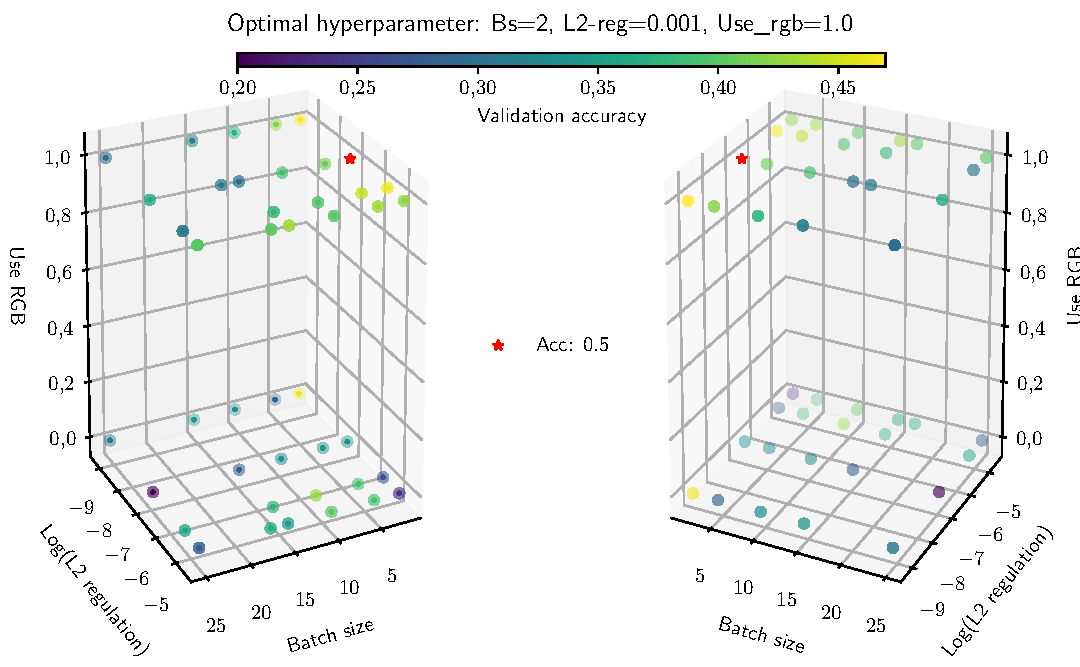
\includegraphics[width=0.5\textwidth]{../../final_data/MiniNN_n5/hyper_raum.pdf}
\caption{Ergebniss der HPO, die $z$-Achse \emph{Use RGB} gibt an, ob Farbinformation
          verwendet wurden. Aus den möglichen Paramtern ist die bestmögliche Kombination
         lautet: $bs=2, \, l2\ua{value}=0.001, \, color=rgb$.}
\label{fig:Hyperraum_MiniDogNN}
\end{figure}
Von den $48$ möglichen Kombinationen wurden $43$ erfolgreich beendet, die Restlichen
wurden auf Grund von Grafikspeicherproblem von \textsc{keras} abgebrochen. Eine
Genauigkeitsverteilung ist in Abbildung \ref{fig:Genauigkeitverteilung_MiniDogNN}
dargestellt. Diese verdeutlicht, dass mit HPO
eine Genauigkeitssteigerung bewirkt werden kann. Der Einfachheit halber wird
angenommen, dass das Ergebnis der HPO, trotz anderem
FCN, sowohl für das fünf als auch für das $120$ Rassen \textsc{MiniDogNN} gilt.

In Abbildung \ref{fig:MiniDogNN_Loss_Acc} findet sich die Traningsdokumentation,
des optimierten Modells. In dem Plot \ref{fig:MiniDogNN_Loss_Acc} ist zu erkennen,
dass die Architektur geringfügig Übertraniertwurde.
Bei Betrachtung der Confusionmatrix in Abbildung \ref{fig:MiniDogNN_Konfusionmatrix} fällt auf, \textbf{dass}
\begin{figure}
\centering
\begin{subfigure}{0.48\textwidth}
\centering
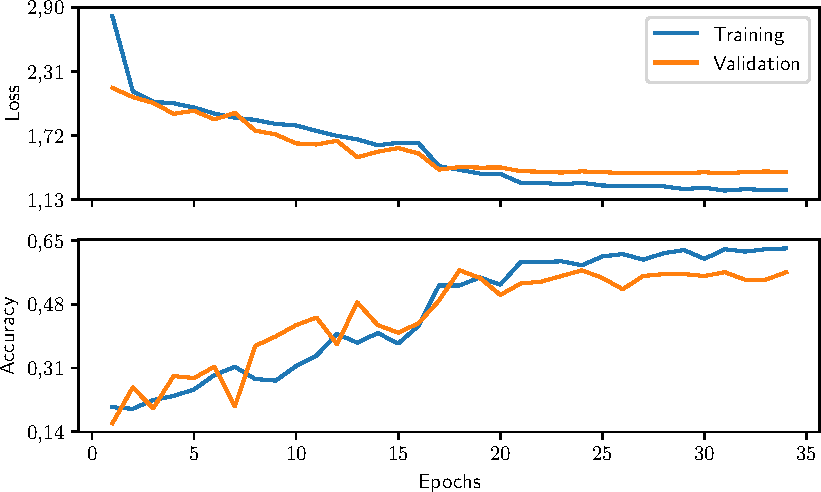
\includegraphics[width = \textwidth]{../../final_data/MiniNN_n5/history.pdf}
\caption{Traningsfortschritt des \textsc{MiniDogNN}.}
\label{fig:MiniDog8NN_Loss_Acc}
\end{subfigure}
\begin{subfigure}{0.48\textwidth}
\centering
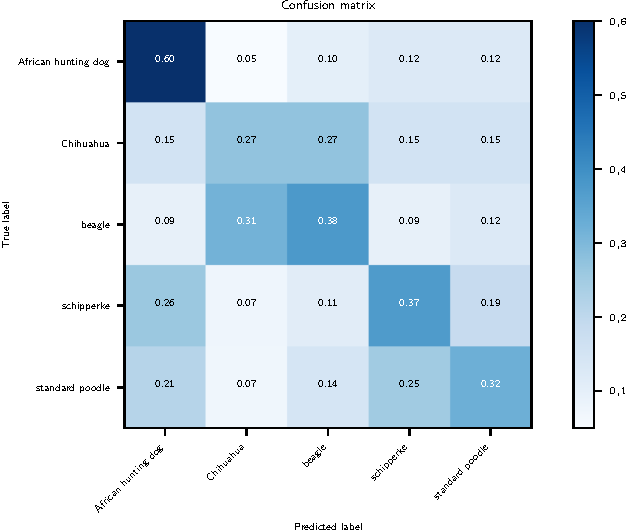
\includegraphics[width = \textwidth]{../../final_data/MiniNN_n5/confusion_matrix.pdf}
\caption{Konfusionmatrix des \textsc{MiniDogNN}.}
\label{fig:MiniDogNN_Konfusionmatrix}
\end{subfigure}
\end{figure}

\subsubsection{PreDogNN -- $5$ Hunderassen}
Die \textsc{PreDogNN}-Architektur wurde mit einer Batachgröße von $16$, einer
$l2$-Regularisierungsstärke von $l2\ua{value}=0.01$, einer Lernrate von
$lr=0.001$, einer Dropourate von $dr=0.2$ und als Farbmodus $color=rgb$ gewählt.
Auf Grund der Verwendung von Dropout muss der Loss und die Genauigkeit nach jeder
Epoche berechnet werden, da sich durch Dropout die Struktur des Netzes epochenweise
ändert. Die resultierenden Loss- und Genauigkeitverläufe befinden sich in Abbildung
\ref{fig:PreDogNN_Loss_Acc}. Die Konfusionmatrix ist in Abbildung \ref{fig:PreDogNN_Konfusionmatrix}
dargestellt. Bemerkenswert ist die Genauigkeit der Architektur welche fast
 bei $100\%$ liegt und somit das \textsc{MiniDogNN} überbietet.
\begin{figure}
\centering
\begin{subfigure}{0.48\textwidth}
\centering
\includegraphics[width = \textwidth]{../../final_data/PreDogNN/16-07-2019_18:39:02/build/history_epoch.pdf}
\caption{Traningsfortschritt des \textsc{PreDogNN}.}
\label{fig:PreDogNN_Loss_Acc}
\end{subfigure}
\begin{subfigure}{0.48\textwidth}
\centering
\includegraphics[width = \textwidth]{../../final_data/PreDogNN/16-07-2019_18:39:02/build/confusion_matrix.pdf}
\caption{Konfusionmatrix des \textsc{PreDogNN}.}
\label{fig:PreDogNN_Konfusionmatrix}
\end{subfigure}
\end{figure}

\subsubsection{MiniDogNN -- $120$ Hunderassen}
Wie in der Abbildung \ref{fig:MiniDogNN} zu erkennen, ändert sich mit der
Anzahl der Hunderassen die Anzahl der Neuornen im FCN. Die Anzahl der generierten
Featuers bleibt jedoch konstant. Ein Fakt der sich siginifikant auf die
Verwendebarkeit der Architektur auswirkt. Bei dem Vergleich mit der Konfusionmatrix
(vgl. Abb. \ref{fig:MiniDogNN_120_Konfusionmatrix}) und
der Loss- und Genauigkeitsdokumentation (vgl. Abb. \ref{fig:MiniDogNN_120_Loss_Acc})
wir deutlich, dass die Architektur kein verwendbare Aussage trifft.

\subsubsection{PreBigDogNN -- $120$ Hunderassen}
Die enorme Anzahl an Features in Verbindung mit der Regularisierung führen dazu,
dass \textsc{PreBigDogNN} eine Genauigkeit deutlich über der Rategenauigkeit
von $0.83\%$ erreicht wird. Hierbei läuft das Modell nur geringfügig in Overtraning,
wie die Traningsdokumentation (vgl. Abb. \ref{fig:PreBigDogNN_Loss_Acc}) zeigt.s
\begin{figure}
\centering
\begin{subfigure}{0.48\textwidth}
\centering
\includegraphics[width = \textwidth]{../../final_data/PreBigDogNN/17-07-2019_12:32:09/build/history_epoch.pdf}
\caption{Traningsfortschritt des \textsc{PreBigDogNN}.}
\label{fig:PreBigDogNN_Loss_Acc}
\end{subfigure}
\begin{subfigure}{0.48\textwidth}
\centering
\includegraphics[width = \textwidth]{../../final_data/PreBigDogNN/17-07-2019_12:32:09/build/confusion_matrix.pdf}
\caption{Konfusionmatrix des \textsc{PreBigDogNN}.}
\label{fig:PreBigDogNN_Konfusionmatrix}
\end{subfigure}
\end{figure}

\subsection{Alternative Methode-- AutoEncoder \& Randomforest -- $120$ Hunderassen}
Der schematische Aufbau des Autoencoder findet sich in Abbildung \ref{fig:Autoencoder}.
Wie dort angedeutet, werden die Bilder auf eine Größe von $96x96$ runterskaliert.
Hierdurch wird kein Bild hochskaliert und die Größe des Featurevektor


. Hiemit soll die Traningszeit des Autoencoders
minimiert werden. Analog zu NN verwendet der Autoencoder auch \textsc{EarlyStopping}
und eine adaptive Lernrate. Der Autoencoder wird traniert mit einer Batchgröße
von $bs=16$ und einer anfänglichen Lernrate von $lr=0.001$. Der Autoencoder
erreicht eine Genauigkeit von $78\%$ (vgl. Abb. \ref{}). Obwohl der Epochenverlauf
der Genauigkeit nicht auf overtraning hindeuten, zeigt sich bei der Losskurve
(vgl. Abb. \ref{}) deutliches overtraning. Dies ist wahrscheinlicha auf die
Verwendung von \textbf{Anzahl Paramter} ohne Regularisierung zurückzuführen.

Mit Hilfe der Features generiert vom Autoencoder soll der
Randomforest (RF) fähig sein Hunderassen zu klassifizieren.
Hierfür wird zunächst eine HPO an einem RF der fünf Hunderassen klassifizieren kann
durchgeführt. Die zu optimierenen Paramter
wurden dem Online-Guide \cite{RF_parameterraum} entommen. Ingesamt
wurd die maximale Tiefe $max_d$, die Methode zu Bestimmung der maximale Anzahl die pro Schnitt verwendet werden
$n\ua{feat}$, die mindest Anzahl an Bildern die einen Ast haben muss, um berücksichtigt zu werden
$min\ua{leaf}$, die mindest  Anzahl an Bildern um einen neuen Ast zueröffnen $min\ua{split}$,
das Bewerungskrietrim $crit$ und die Anzahl der Bäume $n\ua{est}$.
Eine vollständige Auflistung des Parameterraums findet sich in der Gleichung \eqref{eq: rf_parameter_raum}.
\begin{align}
  \begin{aligned}
    \label{eq: rf_parameter_raum}
    max_d &\in \left\{\infty,\, 10,\, 100\right\} & n\ua{feat}&\in\left\{auto, \,log2\right\}\\
    min\ua{leaf} &\in \left\{1,\, 10,\, 31\right\} & min\ua{split}&\in\left\{2,\, 8,\, 10\right\}\\
    crit &\in \left\{gini,\, entropy\right\} & n\ua{est}&\in\left\{100,\, 400,\, 1000,\, 1500 \right\}
  \end{aligned}
\end{align}
Als optimale Parmeter gehenen hervor:
\begin{equation*}
  max_d = 100,\,\, n\ua{feat}= log2, \,\, min\ua{leaf}= 1,\,\, min\ua{split}=10, \,\,   crit= gini, \,\, n\ua{est}=1000
\end{equation*}
Für die Bestimmung der Genauigkeit des RF wird eine CrossValidation mit
drei Iterationen verwendet. Unter der Verwendung der Standartparamter wird eine
erzielt der RF eien Genauigkeit von $acc\ua{default}=43\pm6\%$ erreicht.
Im Vergleich dazu erzielte das optimierte Modell eine Genauigkeit von $acc\ua{opt}=44\pm4\%$.
Die HPO hat in diesem Fall einen geringen Einfluss auf die Genauigkeit des RF,
und sorgt lediglich für eien Verbesserung von $1\%$ und eine geringere Streuung
der mittleren Genauigkeit.
Die Confusionmatrix für die $120$ Rassenklassifzierung ist in Abbildung
\ref{fig:Confusionmatrix_rf} gezeigt. Die mittlere Genauigkeit für den
RF beträgt in diesem Fall $acc\ua{mean,120}=5\pm0.1\%$.
\begin{figure}
\centering
\includegraphics[width=0.5\textwidth]{../../final_data/autoencoder_n_120/build/confusion_matrix.pdf}
\caption{Konfusionmatrix des Randomforest. Der Legendenschlüssel findet sich in
Abbildung \ref{tab:legende_rf}.}
\label{fig:Confusionmatrix_rf}
\end{figure}
